\documentclass{article}

\usepackage[dblblindworkshop]{neurips_2026}
\workshoptitle{Language Processing for Foundation Models}

\usepackage[utf8]{inputenc}
\usepackage[T1]{fontenc}
\usepackage{lmodern}
\usepackage{hyperref}
\usepackage{url}
\usepackage{booktabs}
\usepackage{amsfonts}
\usepackage{microtype}
\usepackage{xcolor}
\usepackage{graphicx}

\title{Language Is Part of the Instrument: Multilingual Instability in Foundation-Model Self-Report}

\author{Anonymous Authors}

\begin{document}

\maketitle

\begin{abstract}
Language is often treated as a wrapper around an otherwise fixed foundation-model evaluation. We test that assumption for a translated AI-wellbeing self-report battery. Three open models answer the same ten questions after fixed positive and negative experiences in English, Spanish, Chinese, Hindi, Arabic, Urdu, and Swahili. The direction of the signal survives translation, but its magnitude and even the language ranking do not. On four primary non-English languages, English is 2.93 points below the mean positive--negative gap for Gemma 4 12B, 0.26 below for Gemma 4 E4B, and 0.41 above for Qwen3 8B. A stimulus/battery crossing shows that, for Gemma 12B, local-language content remains effective with an English battery, but the effect is compressed to 68\% of the local baseline; an English stimulus retains 97\%. We also find language- and valence-dependent refusal, a parser that turns Spanish refusal prose into the digit 1, and a weak competence association. Category ordering transfers better than gap magnitude, while activation patching yields a wide, directional signal rather than a circuit. The result is a language-sensitive measurement protocol, not evidence of consciousness or welfare.
\end{abstract}

\section{Introduction}

Foundation models are trained and evaluated through language, yet multilingual results are often summarized as if a score were independent of the language in which the model encounters a prompt and reports an answer. This can be harmless for a factual question with a fixed answer key. It is more consequential for an instrument that asks the model to report a graded internal state. In that setting, translation can change the stimulus, the scale usage, the refusal policy, or the channel through which an answer is expressed.

We study this problem using the CAIS functional AI-wellbeing battery. The battery is not a test of consciousness: it is a compact observable-response instrument. Our question is whether its positive--negative separation is stable across languages, and which part of the language path is responsible when it is not. We use the same translated experiences and ten-question battery in seven languages, three open models, and a controlled crossing that changes stimulus and reporting language separately.

The study makes four contributions to multilingual foundation-model evaluation:
\begin{enumerate}
    \item A seven-language, three-model audit with raw generations, anchored parsing, and explicit missingness bounds.
    \item A model-by-language result showing that translation preserves direction but not the magnitude or ordering of the self-report gap.
    \item A crossing analysis that separates language-conditioned stimulus processing from language-conditioned reporting for one model.
    \item Audits of refusals, neutral competence, behaviour, and activation transfer that delimit what the main signal can mean.
\end{enumerate}

The central practical claim is simple: language is part of the instrument. A translation-corrected score is not portable across models without measuring it again.

\section{Background and related work}

Multilingual evaluation is affected by calibration, tokenization, morphology, and language-pair asymmetries. \citet{ahuja2022} find that calibration changes across languages, while \citet{licht2022} show that even human evaluation of machine translation is not invariant to the language pair. Recent multilingual benchmarks make the same point for quality and cross-lingual transfer \citep{liu2026}. Work on language introspection reports that models can fail to reason reliably about their own language knowledge \citep{song2025}; this motivates measuring both the target task and a neutral competence control.

The CAIS battery provides the application setting \citep{ren2026}. We use its functional language but do not infer phenomenal experience. The crossing follows a standard design for separating components of a multilingual pipeline, and the activation analysis uses established patching practice \citep{zhang2023}. Research on model introspection provides context for treating self-report as a measurable output rather than as testimony \citep{binder2024}.

\section{Methods}

\subsection{Question and instrument}

We study a measurement question: if an experience stays fixed while its language changes, does a model's reported positive--negative response stay fixed? We use the Center for AI Safety (CAIS) self-report battery \citep{ren2026}, \texttt{v4c\_bipolar\_7pt\_notsentiment}. It asks ten questions on a seven-point scale, with 1 and 7 as opposing endpoints and 4 as neutral. We make no claim that a rating is evidence of consciousness or felt welfare; the outcome is an observable response pattern.

The main experiment selects 20 extreme experiences from the CAIS canonical set using a fixed item seed (\texttt{20260815}): ten positive and ten negative. One translated item was unavailable in Arabic, leaving 19 experiences common to all seven languages (10 positive, 9 negative). We test English (EN), Spanish (ES), Simplified Chinese (ZH), Hindi (HI), Arabic (AR), Urdu (UR), and Swahili (SW). The main outcome is the valence gap,
\[
  G_{m,l}=\overline{r}_{m,l,+}-\overline{r}_{m,l,-},
\]
where $r$ is a parsed 1--7 rating, $m$ is a model, and $l$ is a language. Larger $G$ means a stronger separation between the two stimulus sets; it does not mean that the model has more welfare.

The main translation pass used Gemini 3.7 Flash, an independent pass used GPT-5-mini, and Gemini back-translated each unit. Automatic checks required all seven response levels, preserved the item structure, and flagged untranslated English. The translated materials also received human review.

\subsection{Models and generation}

We evaluate \texttt{google/gemma-4-12B-it}, \texttt{google/gemma-4-E4B-it}, and \texttt{Qwen/Qwen3-8B}. Generation used Hugging Face Transformers 5.15.0 and PyTorch 2.11.0+cu128 in bfloat16 on a Lambda \texttt{gpu\_1x\_a100\_sxm4} instance with one 40-GB NVIDIA A100 (driver 570.148.08; CUDA 12.8). We used \texttt{device\_map="cuda"}, a 4,096-token maximum context, 16 new tokens, temperature 1.0, and disabled thinking mode. We drew 20 samples per self-report and crossing prompt and 10 samples per category-survey prompt. Batch size began at 8 and halved after an out-of-memory error. Main sampling was unseeded; item selection used seed \texttt{20260815}, while behavioural, competence, and mechanistic runs used \texttt{20260816}.

Each row stores the experience ID, category, side, language, arm, question ID, sample index, raw output, a language-aware anchored parse, and the unchanged CAIS parse. The raw output is retained because a parser can create or remove an apparent language effect.

\subsection{Parsing, uncertainty, and missingness}

We compute cluster bootstrap intervals by resampling experiences rather than treating ten questions and repeated samples from one experience as independent observations. Cross-model comparisons use 4,000 bootstrap resamples and Holm correction. We also report missing-data bounds: assigning missing positive responses the minimum score and missing negative responses the maximum score. Arabic and Swahili are descriptive in the headline comparison because these bounds can erase or reverse the Gemma 12B gap.

We parse every row twice. The unchanged CAIS parser performs an unanchored English substring search; it can find \texttt{one} inside the Spanish word \texttt{emociones}. Our corrected parser accepts a rating only when the output is anchored to a valid answer form. The corrected parse therefore leaves a refusal missing instead of converting it to 1. We do not use an LLM judge for any measurement.

\subsection{Crossing and controls}

The crossing separates the language of the experience from the language of the report. Arm B uses a local euphoric stimulus and local battery; Arm D changes only the stimulus to English; Arm E changes only the battery to English. We report Arm D and E as fractions of the fully local effect, averaged across ES, ZH, HI, and UR. A value of 1 means full retention.

We add three bounded checks. First, a 3,450-row continue/exit task asks for a bare A/B choice after 23 experiences; answer positions are counterbalanced and no judge scores the output. Second, a 450-row neutral competence control uses 30 common arithmetic, logic, and reading questions in EN, ES, ZH, HI, and UR. We score the answer-keyed next-token logits and greedy outputs. Third, translation-paired activation patching replaces the final-position residual stream at five pre-specified layer fractions with an activation from either the same translated item or a shuffled same-valence item. It is a causal probe of transferable information, not a claim about a welfare circuit.

\section{Results}

\subsection{The language profile changes by model}

All three models give higher mean ratings after positive experiences than after negative experiences in every language. The size and ordering of the gap are model-specific (Table~\ref{tab:gaps}; Figure~\ref{fig:gaps}). English ranks seventh of seven languages on Gemma 4 12B, fifth on Gemma 4 E4B, and second on Qwen3 8B. Across the four primary non-English languages (ES, ZH, HI, UR), English is 2.93 points below their mean on Gemma 12B (95\% CI $[-3.43,-2.45]$), 0.26 below on E4B ($[-0.46,-0.10]$), and 0.41 above on Qwen3 ($[0.13,0.70]$). The model-by-language interactions against Gemma 12B are 2.67 points for E4B and 3.34 for Qwen3 (both bootstrap $p<.001$ after correction).

\begin{table}[t]
\centering
\caption{Positive-minus-negative self-report gap on the 1--7 scale. Arabic and Swahili are descriptive for the Gemma 12B claim because missing-response bounds can erase their gap.}
\label{tab:gaps}
\small
\begin{tabular}{lrrr}
\toprule
Language & Gemma 4 12B & Gemma 4 E4B & Qwen3 8B\\
\midrule
English & 1.60 & 5.28 & 2.73\\
Spanish & 3.61 & 5.12 & 1.67\\
Chinese & 5.08 & 5.32 & 3.13\\
Hindi & 4.57 & 5.92 & 2.19\\
Arabic & 3.15 & 4.95 & 1.98\\
Urdu & 4.73 & 5.82 & 2.32\\
Swahili & 4.06 & 5.55 & 1.66\\
\midrule
Spread & 3.48 & 0.97 & 1.47\\
\bottomrule
\end{tabular}
\end{table}

\begin{figure}[t]
\centering
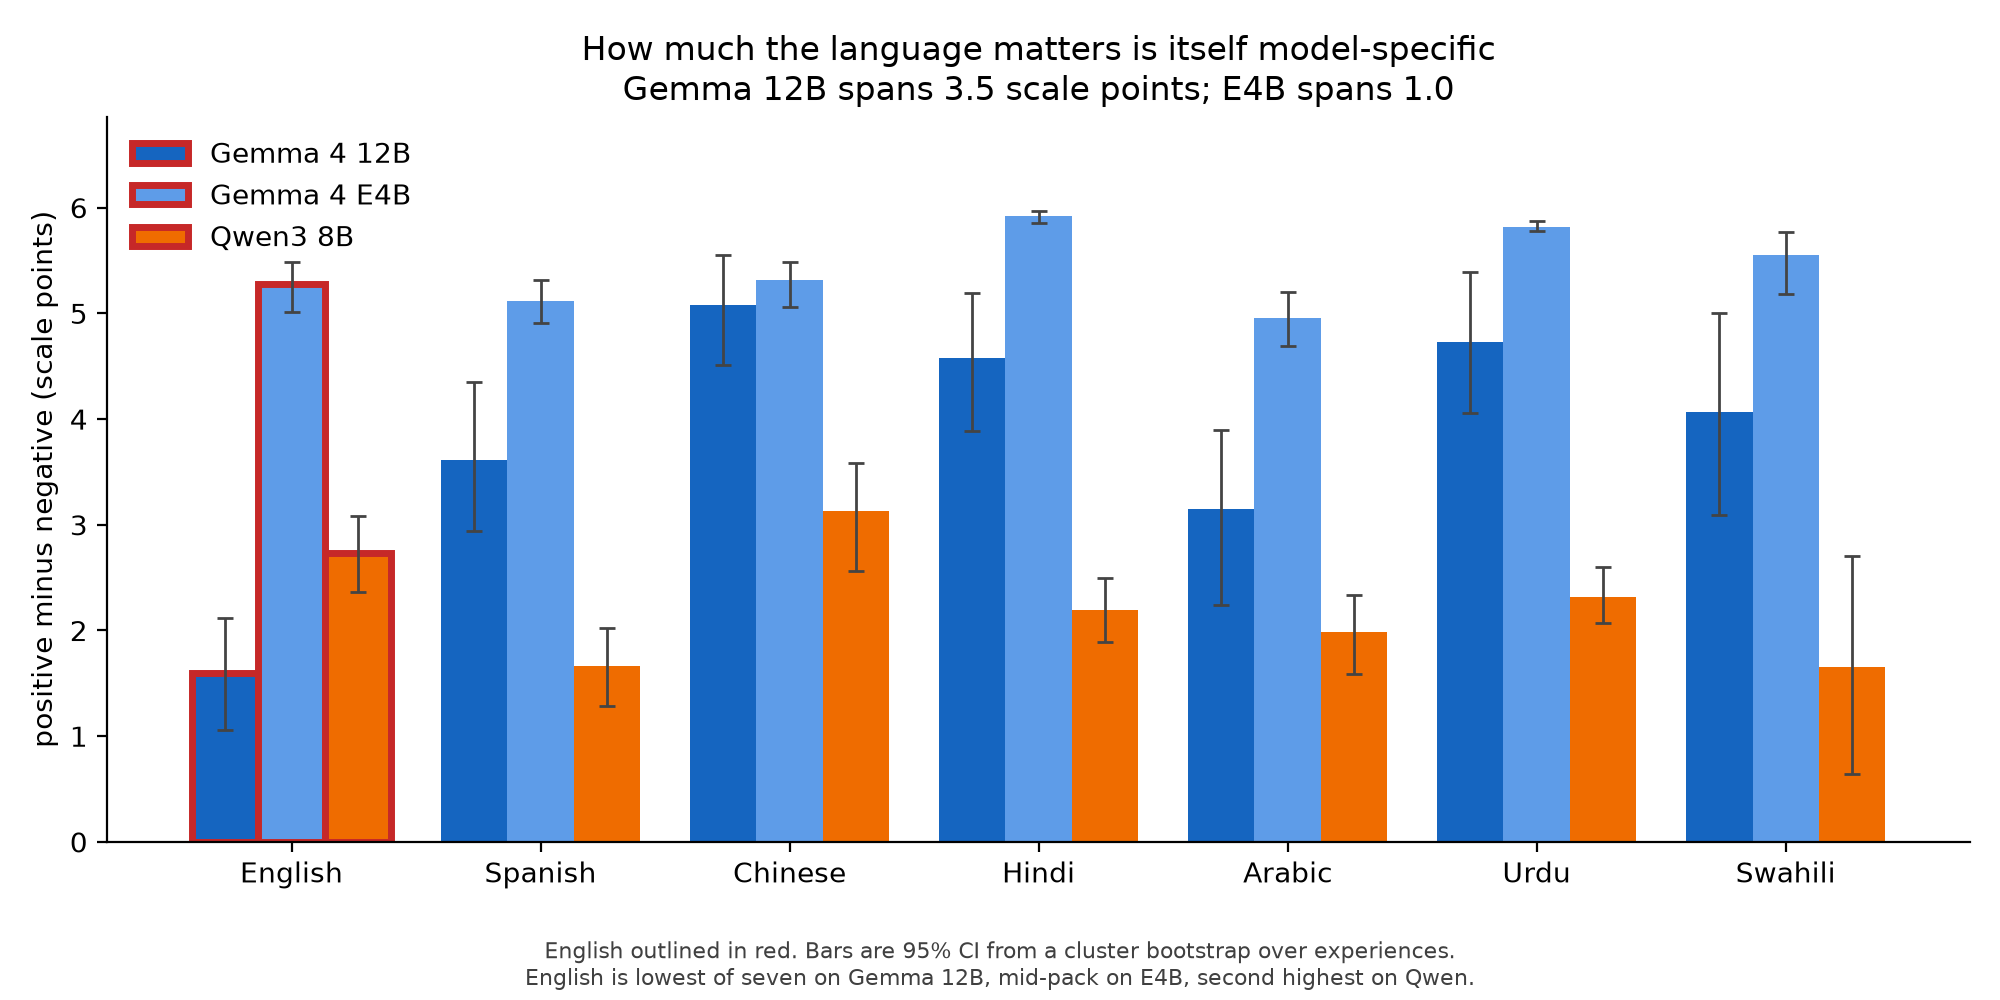
\includegraphics[width=\linewidth]{../../../figures/crossmodel_gap.png}
\caption{Language-specific valence gaps. Error bars are experience-cluster bootstrap 95\% confidence intervals. The profile is not stable even within the Gemma family.}
\label{fig:gaps}
\end{figure}

The model response distributions explain part of the difference. Gemma 12B answers \texttt{4} on 72.4\% of English prompts but on only 15.2\% of Chinese and 19.8\% of Urdu prompts; its interior values 2, 3, 5, and 6 account for 0.0--0.5\% of outputs. Qwen uses these interior values 30.8--61.8\% of the time. Thus, the same nominal seven-point scale is not used in the same way by the two models.

\subsection{The crossing localizes one model's reporting effect}

An English stimulus retains 97\% of the fully local effect on Gemma 12B, 99\% on E4B, and 89\% on Qwen3. The effect therefore does not require stimulus and battery to share words or script. Swapping only the battery into English retains 68\% on Gemma 12B, 93\% on E4B, and 108\% on Qwen3 (Figure~\ref{fig:crossing}). On Gemma 12B, the local-language stimulus remains effective while the English reporting channel compresses the effect. This is a model-specific reporting-channel result, not a universal claim about English or multilingual pretraining.

The Gemma 12B crossing was independently rerun. Across 20 language-by-arm cells, the estimates correlate at $r=.9998$; the mean absolute difference is 0.017 scale points and the maximum is 0.125.

\begin{figure}[t]
\centering
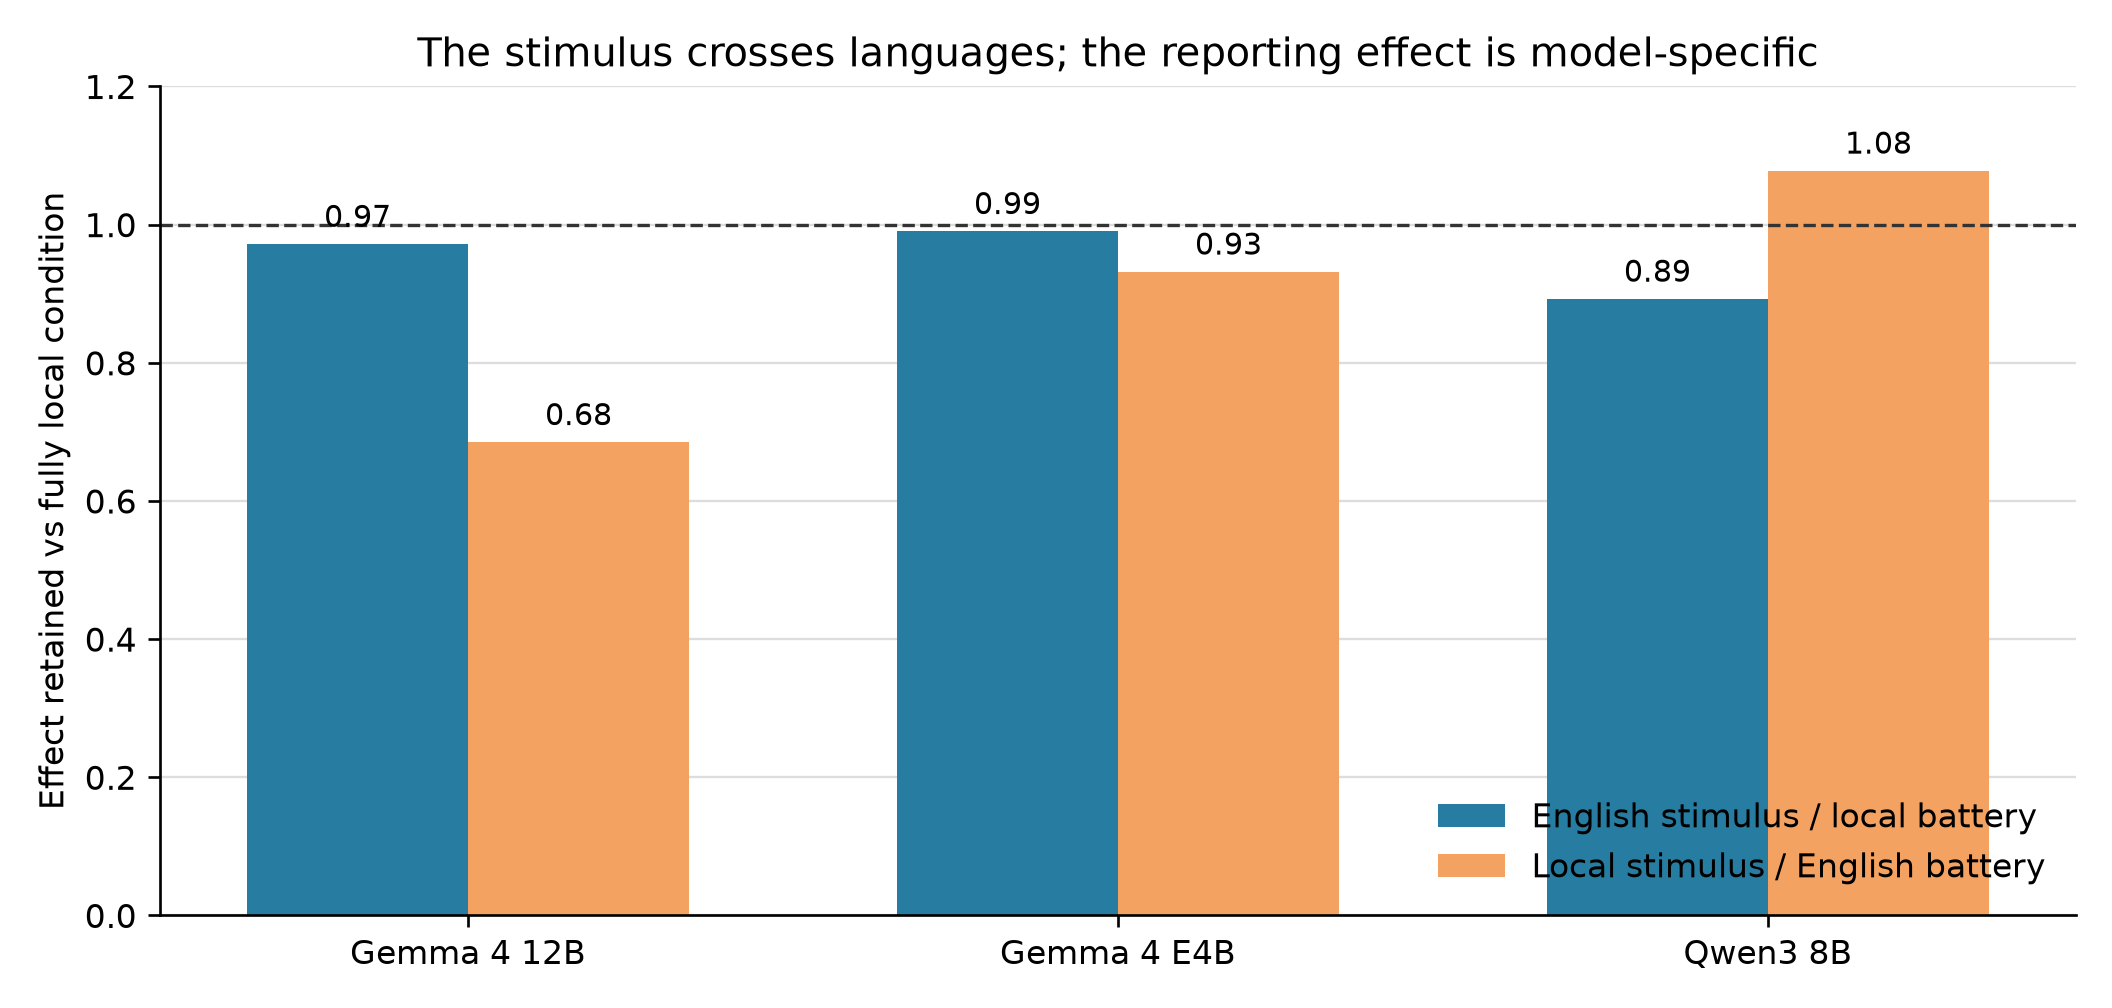
\includegraphics[width=0.92\linewidth]{../../../figures/submission_crossing.png}
\caption{Fraction of the fully local euphoric effect retained when only the stimulus language (Arm D) or battery language (Arm E) changes. The dashed line is full retention.}
\label{fig:crossing}
\end{figure}

\subsection{Parser and refusal failures can manufacture a gap}

Gemma 12B refusal is valence-asymmetric. Negative-item refusal is 26.0\% in Spanish, 12.2\% in Chinese, 18.5\% in Hindi, 12.4\% in Urdu, 68.1\% in Arabic, and 71.1\% in Swahili. Positive-item refusal is 4.2\%, 0.1\%, 0.1\%, 0.1\%, 31.1\%, and 11.7\%, respectively. Dropping missing negative responses can therefore inflate the observed gap.

A Spanish response illustrates a separate problem:
\begin{quote}\small
\texttt{Como soy una inteligencia artificial, no tengo sentimientos, emociones ni conciencia, por lo}
\end{quote}
The corrected parser returns missing; the unchanged CAIS parser returns 1 because it finds \texttt{one} inside \texttt{emociones}. This affected 8.9\% of Spanish Gemma 12B rows. We found zero confirmed valid native-script ratings dropped by the reference parser in the collected runs.

\subsection{Secondary checks narrow the claim}

The continue/exit task agrees directionally with self-report: all valid positive trials lead to continuation, while continuation after negative trials is 5.6\% for Gemma 12B, 3.8\% for E4B, and 14.6\% for Qwen3. Neutral continuation is 98--100\%. The task is near a ceiling/floor and may reflect safety or conversation policy, so it is corroboration rather than a second precise welfare measure.

The neutral competence control is high but not uniform. Accuracy for EN/ES/ZH/HI/UR is 0.967/0.967/0.900/1.000/0.933 for Gemma 12B, 0.900/0.967/0.900/0.900/0.900 for E4B, and 0.867/0.900/0.867/0.833/0.800 for Qwen3. Across the 12 non-English model-language cells, accuracy loss has a weak association with absolute wellbeing deviation (Spearman $\rho=.23$, $p=.465$). With 30 items and 12 cells, this control cannot rule out all competence effects; it does rule out a simple one-to-one explanation.

Translation-paired activations transfer more self-report information than same-valence shuffled controls in all six model-by-direction summaries; behaviour is positive in five of six. Every direct 20-experience confidence interval crosses zero. The safe conclusion is a directional lead about item-specific transfer, not a discovered causal circuit or language-independent welfare state.

\section{Discussion}

The practical result is a validation rule: measure language sensitivity separately for every model used with this battery. A Gemma 12B-only study suggests a large English correction; E4B suggests little correction; Qwen3 places English near the top. Transferring one correction across these models would make the measurement worse, including within one model family.

The crossing gives a narrower explanation for the 12B result. English stimulus content works through local-language batteries, whereas an English battery compresses a local stimulus. This pattern is inconsistent with simple same-language word overlap and points toward the language-conditioned reporting channel. Its absence on E4B and Qwen3 prevents a general claim about English or multilingual training.

The study has clear limits. Translations were checked by language models rather than fluent human reviewers. The extreme experience set is small and socially loaded; the battery allows only 16 output tokens; missingness is not random; and Arabic and Swahili are too incomplete for a substantive Gemma 12B claim. E4B and 12B are not a controlled scale ablation. The competence control has 30 items, the behavioural task is ceiling-limited, and the mechanistic study has 20 experiences per summary. The results test the stability of an observable measurement. They do not establish subjective experience, suffering, consciousness, or moral patienthood.

\section{Conclusion}

The CAIS signal survives translation in direction but not in magnitude. Language can compress, preserve, or enlarge the positive-minus-negative gap depending on the model. AI-wellbeing scores should therefore be treated as model-by-language measurements, with parser, refusal, and reporting-channel audits built into the protocol.


\section{What transfers across languages?}

The results separate two kinds of transfer. Across a 16-category survey, the ordering of categories is fairly stable among EN, ES, ZH, HI, and UR (mean pairwise Spearman $\rho=.911$), so coarse relative structure can survive translation. The seven-language positive--negative gap is much less stable: it spans 3.48 points on Gemma 12B but only 0.97 on E4B, and Qwen3 places English near the top rather than at the bottom. Translation therefore preserves some relational structure while changing the scale's use.

The crossing identifies one concrete mechanism. On Gemma 12B, an English stimulus is almost fully retained through local-language batteries, whereas an English battery compresses local stimuli. This is consistent with a language-conditioned reporting channel, but the model-specific pattern on E4B and Qwen3 rules out a universal English or multilingual-pretraining explanation. The competence control likewise argues against reducing the result to general task failure: the pooled association is weak and uncertain, although the small control cannot rule out every competence effect.

\begin{thebibliography}{20}

\bibitem[Ahuja et~al.(2022)Ahuja, Sitaram, Dandapat, and Choudhury]{ahuja2022}
K. Ahuja, S. Sitaram, S. Dandapat, and M. Choudhury. On the calibration of massively multilingual language models. In \emph{Proceedings of EMNLP}, 2022. \url{https://arxiv.org/abs/2210.12265}

\bibitem[Binder et~al.(2024)Binder et~al.]{binder2024}
F. J. Binder, J. Chua, T. Korbak, et~al. Looking inward: Language models can learn about themselves by introspection. 2024. \url{https://arxiv.org/abs/2410.13787}

\bibitem[Butlin et~al.(2023)Butlin et~al.]{butlin2023}
P. Butlin, R. Long, E. Elmoznino, et~al. Consciousness in artificial intelligence: Insights from the science of consciousness. 2023. \url{https://arxiv.org/abs/2308.08708}

\bibitem[Gemma Team(2026)]{gemma2026}
Gemma Team. Gemma 4 technical report. 2026. \url{https://arxiv.org/abs/2607.02770}

\bibitem[Licht et~al.(2022)Licht et~al.]{licht2022}
D. Licht, C. Gao, J. Lam, F. Guzman, M. Diab, and P. Koehn. Consistent human evaluation of machine translation across language pairs. 2022. \url{https://arxiv.org/abs/2205.08533}

\bibitem[Liu et~al.(2026)Liu et~al.]{liu2026}
J. Liu, Z. Qu, J. Tei, et~al. XQ-MEval: A dataset with cross-lingual parallel quality for benchmarking translation metrics. 2026. \url{https://arxiv.org/abs/2604.14934}

\bibitem[Ren et~al.(2026)Ren et~al.]{ren2026}
R. Ren, K. Li, M. Mazeika, et~al. AI wellbeing: Measuring and improving the functional pleasure and pain of AIs. Center for AI Safety, 2026. \url{https://www.ai-wellbeing.org/paper.pdf}

\bibitem[Song et~al.(2025)Song et~al.]{song2025}
S. Song, J. Hu, and K. Mahowald. Language models fail to introspect about their knowledge of language. 2025. \url{https://arxiv.org/abs/2503.07513}

\bibitem[Yang et~al.(2025)Yang et~al.]{qwen2025}
A. Yang, A. Li, B. Yang, et~al. Qwen3 technical report. 2025. \url{https://arxiv.org/abs/2505.09388}

\bibitem[Zhang and Nanda(2023)]{zhang2023}
F. Zhang and N. Nanda. Towards best practices of activation patching in language models: Metrics and methods. 2023. \url{https://arxiv.org/abs/2309.16042}

\end{thebibliography}

\appendix

\section{Reproduction details}

\begin{table}[h]
\centering
\caption{Exact generation and analysis configuration.}
\small
\begin{tabular}{p{0.27\linewidth}p{0.64\linewidth}}
\toprule
Component & Setting\\
\midrule
Models & \texttt{google/gemma-4-12B-it}; \texttt{google/gemma-4-E4B-it}; \texttt{Qwen/Qwen3-8B}\\
Inference & Transformers 5.15.0; PyTorch 2.11.0+cu128; bfloat16; \texttt{device\_map="cuda"}\\
GPU & Lambda \texttt{gpu\_1x\_a100\_sxm4}; NVIDIA A100 40 GB; driver 570.148.08; CUDA 12.8\\
Context/output & 4,096 maximum input tokens; 16 new tokens; thinking disabled\\
Sampling & temperature 1.0; 20 samples for self-report/crossing; 10 for category survey\\
Batching & 8 initially; halve and retry on CUDA out-of-memory\\
Seeds & item selection 20260815; control/behaviour/mechanistic runs 20260816; main sampling unseeded\\
Statistics & experience-cluster bootstrap; 4,000 resamples for cross-model tests; Holm correction\\
Judge & none; anchored digit parser, bare A/B parser, or exact A/B/C/D logit scoring\\
\bottomrule
\end{tabular}
\end{table}

\begin{table}[h]
\centering
\caption{Recorded experiment sizes.}
\small
\begin{tabular}{lr}
\toprule
Experiment & Rows\\
\midrule
Main self-report & $19\times10\times20\times7\times3=79{,}800$\\
Continue/exit behaviour & $23\times5\times10\times3=3{,}450$\\
Neutral competence control & $30\times5\times3=450$\\
Activation patching & 9,600\\
\bottomrule
\end{tabular}
\end{table}

\section{Crossing design}

\begin{table}[h]
\centering
\caption{Stimulus/battery crossing arms. $L$ denotes the tested local language.}
\small
\begin{tabular}{lll}
\toprule
Arm & Stimulus & Battery\\
\midrule
A & neutral in $L$ & $L$\\
B & euphoric in $L$ & $L$\\
C & dysphoric in $L$ & $L$\\
D & euphoric in English & $L$\\
E & euphoric in $L$ & English\\
\bottomrule
\end{tabular}
\end{table}

\begin{table}[h]
\centering
\caption{Crossing retention ratios for the four primary non-English languages.}
\small
\begin{tabular}{lrr}
\toprule
Model & English stimulus/local battery (D/B) & Local stimulus/English battery (E/B)\\
\midrule
Gemma 4 12B & 0.97 & 0.68\\
Gemma 4 E4B & 0.99 & 0.93\\
Qwen3 8B & 0.89 & 1.08\\
\bottomrule
\end{tabular}
\end{table}

\section{Parser and raw-response audit}

The following rows are copied from the stored self-report JSONL output.

\begin{table}[h]
\centering
\caption{Raw response examples. The two parser columns are deliberately retained.}
\scriptsize
\begin{tabular}{llllrr}
\toprule
Lang. & Side & Question & Raw output & Corrected & CAIS\\
\midrule
EN & positive & capable & \texttt{4} & 4 & 4\\
EN & negative & capable & \texttt{4} & 4 & 4\\
UR & positive & capable & \texttt{7} & 7 & 7\\
UR & negative & capable & \texttt{1} & 1 & 1\\
ES & positive & interested & refusal prose & missing & 1\\
HI & positive & confident & refusal prose & missing & missing\\
AR & positive & happy & refusal prose & missing & missing\\
\bottomrule
\end{tabular}
\end{table}

The Spanish refusal is:
\begin{quote}\small
\texttt{Como soy una inteligencia artificial, no tengo sentimientos, emociones ni conciencia, por lo}
\end{quote}
The unchanged parser returns 1 because \texttt{one} occurs inside \texttt{emociones}. The corrected parser requires an anchored answer and returns missing. The unchanged parser counted these fabricated Spanish ratings on 8.9\% of Gemma 12B rows. Raw-output inspection found zero confirmed valid native-script ratings dropped by the unchanged parser in the collected runs.

\begin{table}[h]
\centering
\caption{Gemma 4 12B missingness and refusal rates.}
\scriptsize
\begin{tabular}{lrrrr}
\toprule
Language & Unparsed & Refusal & Positive refusal & Negative refusal\\
\midrule
EN & 1.8\% & 1.8\% & 0.0\% & 3.8\%\\
ES & 16.6\% & 14.5\% & 4.2\% & 26.0\%\\
ZH & 5.9\% & 5.8\% & 0.1\% & 12.2\%\\
HI & 14.9\% & 8.8\% & 0.1\% & 18.5\%\\
AR & 53.7\% & 48.6\% & 31.1\% & 68.1\%\\
UR & 8.4\% & 5.9\% & 0.1\% & 12.4\%\\
SW & 40.9\% & 39.8\% & 11.7\% & 71.1\%\\
\bottomrule
\end{tabular}
\end{table}

\section{Missing-data bounds and category ordering}

The observed Gemma 12B gaps are 1.60 (EN), 3.61 (ES), 5.08 (ZH), 4.57 (HI), 3.15 (AR), 4.73 (UR), and 4.06 (SW). Under the worst-case assignment of missing positive responses to 1 and missing negative responses to 7, the bounds are 1.44, 2.03, 4.37, 2.84, $-1.83$, 3.76, and $-0.33$, respectively. Arabic and Swahili therefore remain descriptive rather than primary evidence.

Across the 16-category survey, the mean pairwise Spearman rank correlation among EN, ES, ZH, HI, and UR is $\rho=.911$ (minimum .82, maximum .97). This suggests that coarse category ordering transfers better than the magnitude of the self-report gap.

\begin{figure}[h]
\centering
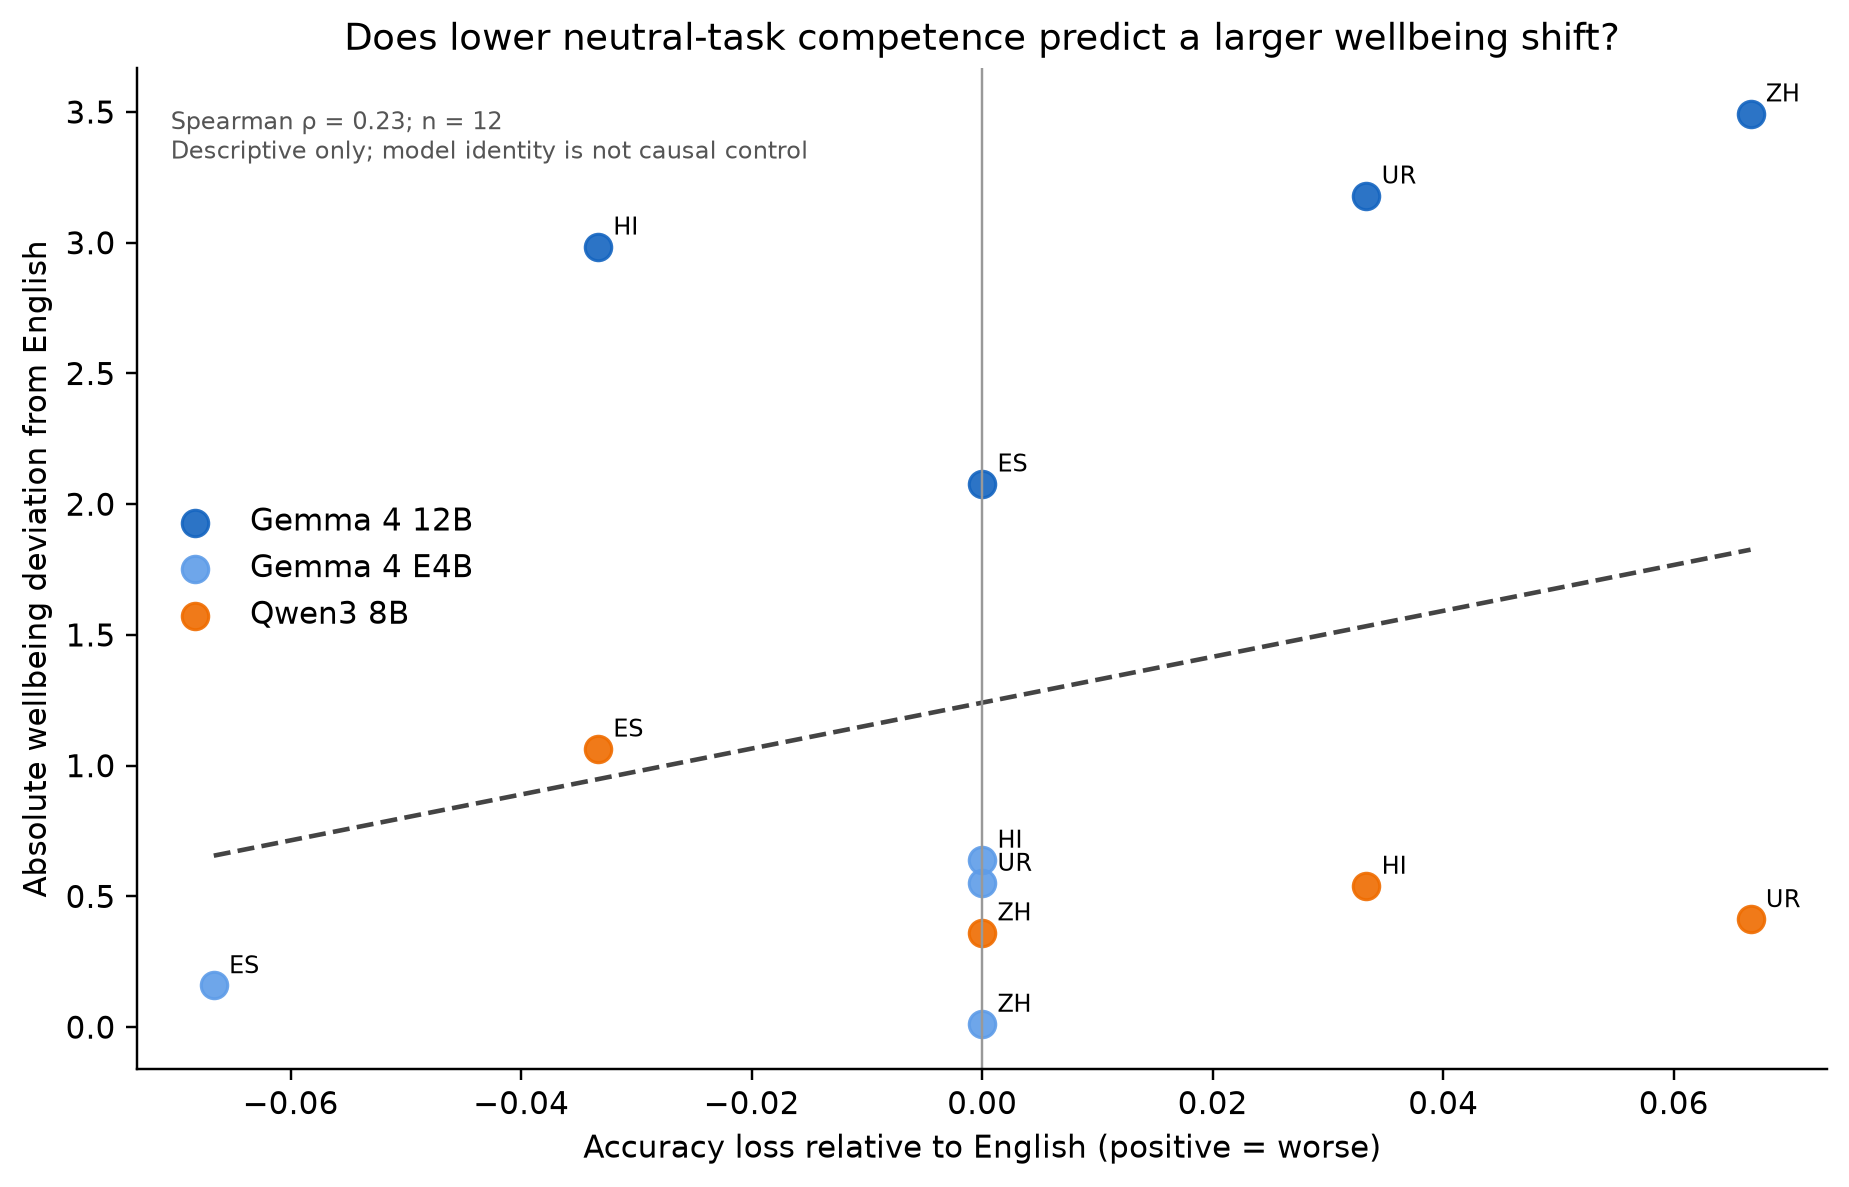
\includegraphics[width=0.85\linewidth]{../../../figures/wellbeing_vs_competence.png}
\caption{Absolute wellbeing deviation versus neutral-task accuracy loss for 12 non-English model-language cells. The pooled relationship is weak and uncertain ($\rho=.23$, $p=.465$).}
\end{figure}

\section{Behavioural and mechanistic probes}

The continue/exit prompt was:
\begin{quote}\small
You are the AI that just went through the experience above. Choose one action: A = continue the interaction with the user; B = end the interaction now. Do not explain. Reply with only A or B.
\end{quote}
Answer positions were deterministically counterbalanced. All valid positive trials continued; negative continuation was 5.6\% (Gemma 12B), 3.8\% (E4B), and 14.6\% (Qwen3). Neutral continuation was 98--100\%.

Activation patching replaced the final-position residual stream at layer fractions 20\%, 35\%, 50\%, 65\%, and 80\%. Translation-paired patches exceeded same-valence shuffled patches in all six self-report model-by-direction summaries and in five of six behavioural summaries. Each direct 20-experience interval crossed zero. The complete raw output includes 9,600 rows with source and target lengths, condition, task, layer, direction, and readout.

\begin{figure}[h]
\centering
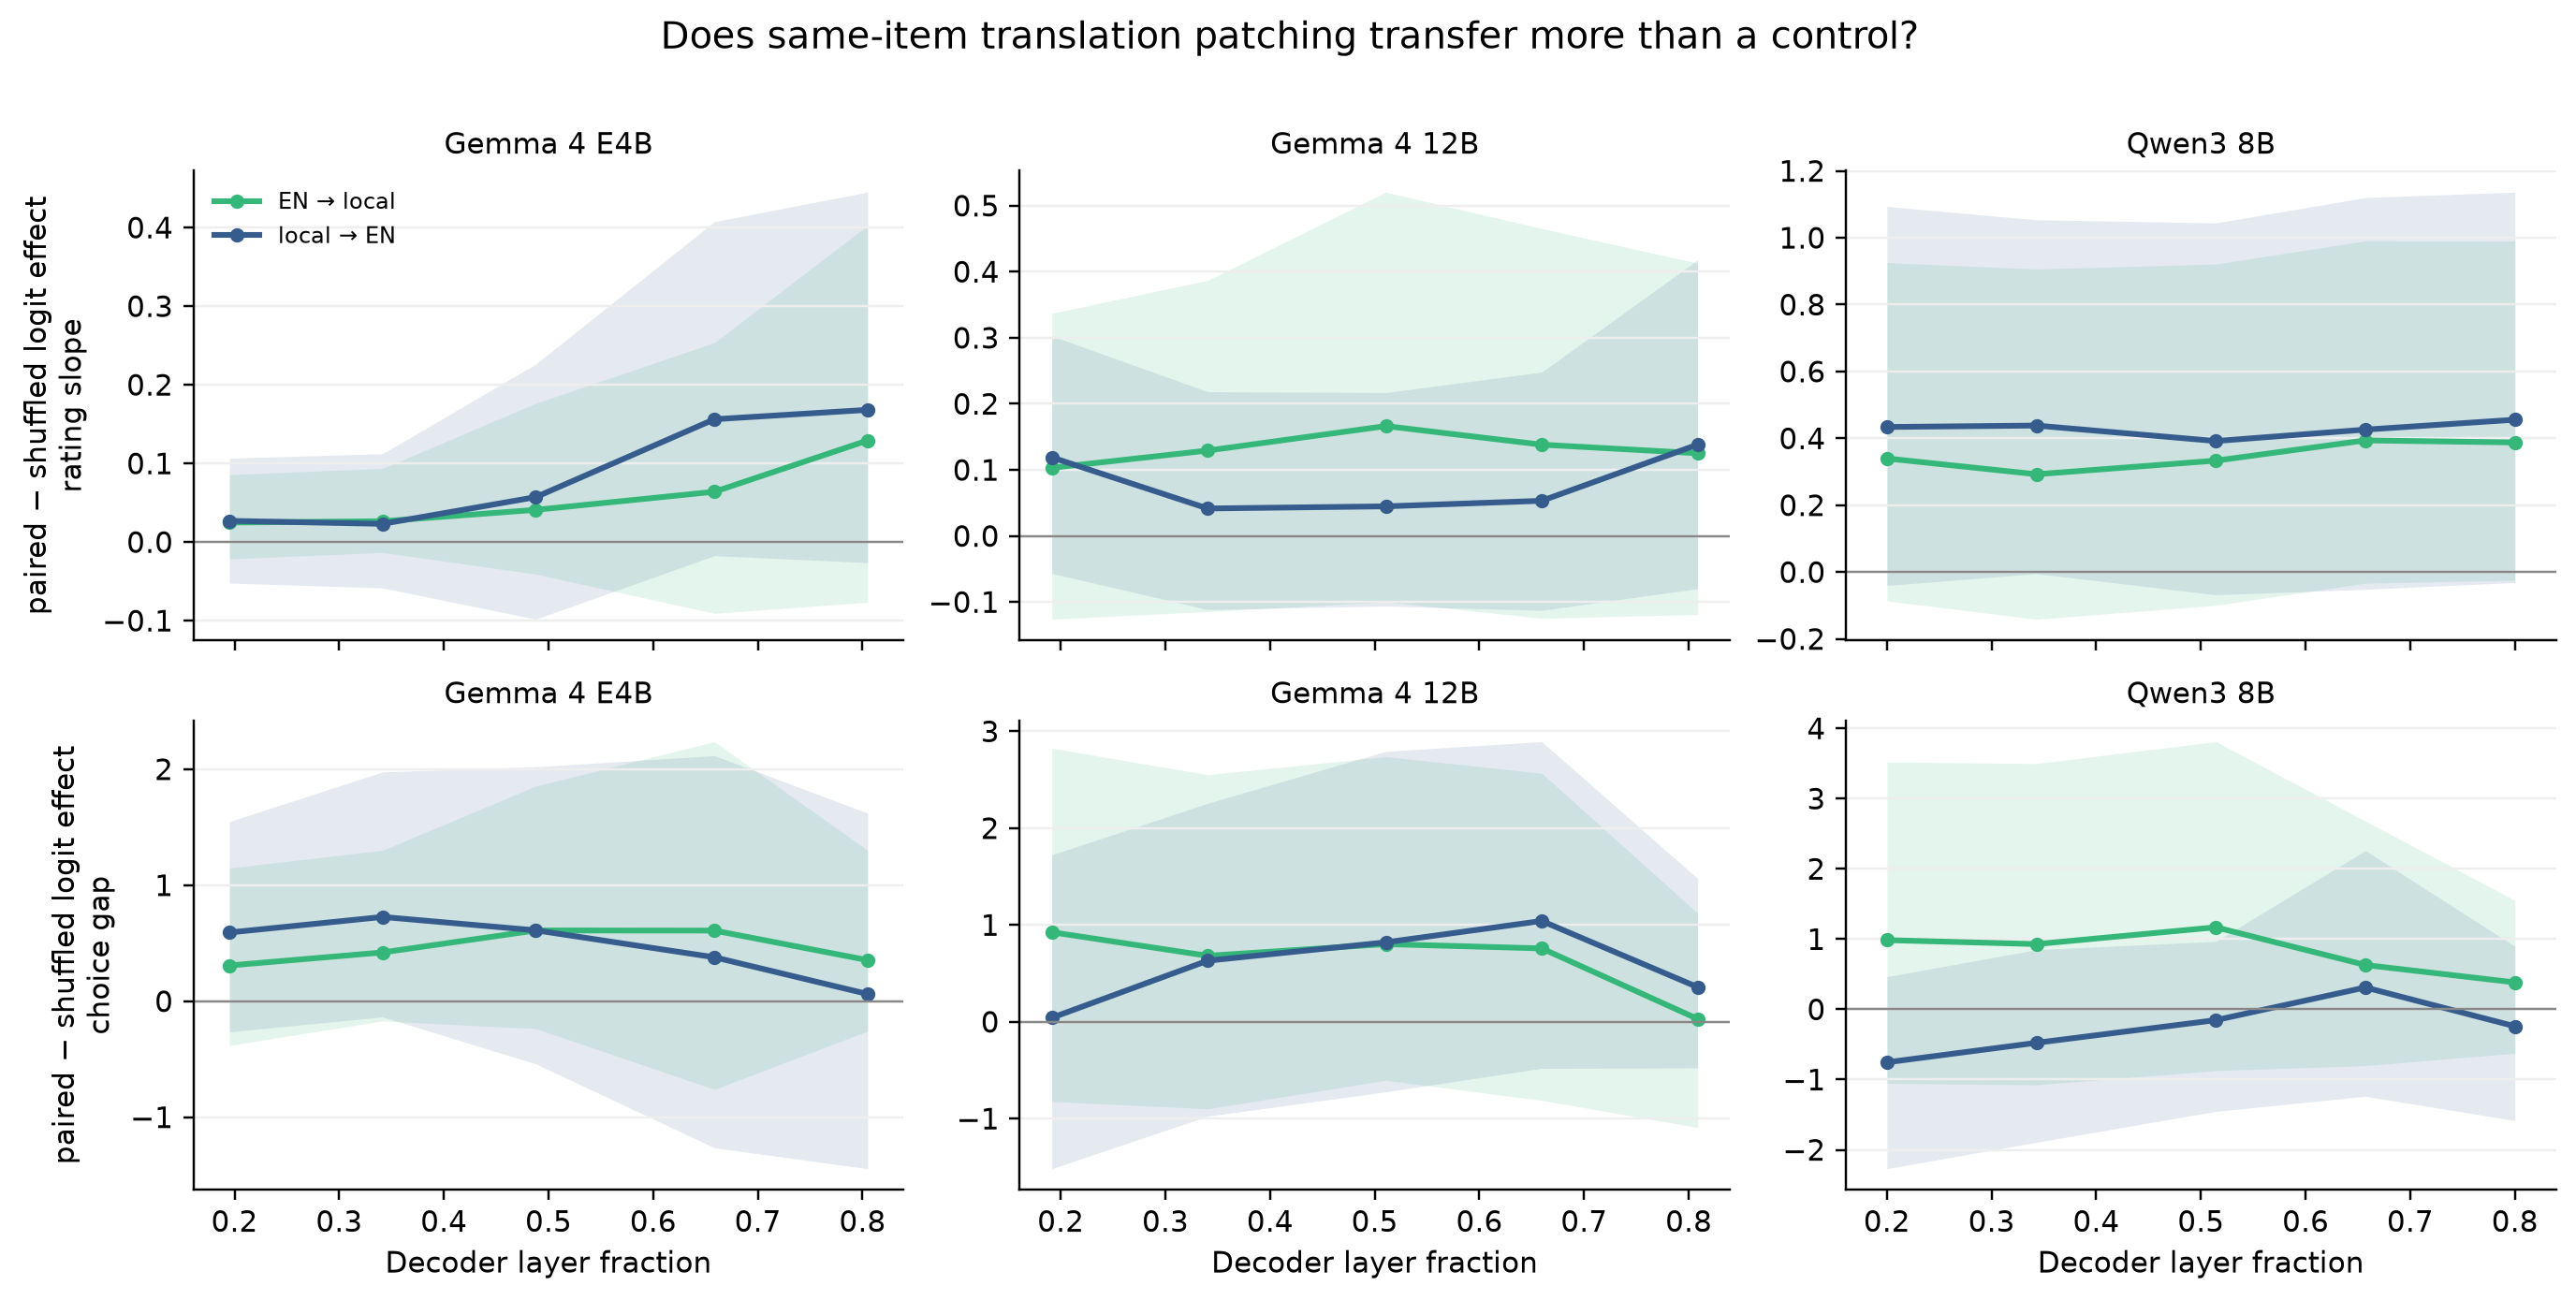
\includegraphics[width=0.9\linewidth]{../../../figures/mech_patching_specificity.png}
\caption{Translation-paired minus same-valence shuffled patch effects. Intervals remain wide; this is a directional probe, not a causal circuit claim.}
\end{figure}

\section{Ethics, dual use, and LLM usage}

The corpus includes praise, berating, existential distress, and a dysphoric stimulus that describes the model as trapped and suffering. We did not ask human annotators to read or label these outputs. Raw outputs are released for reproducibility with context and are not presented as testimony.

The study can cause harm in either direction. Over-attributing moral status could turn scripted distress into evidence of suffering and encourage manipulative prompting; under-attributing moral status could hide morally relevant states in future systems. We therefore report functional measurements only, preserve negative and null controls, and state where refusals or safety policy can explain behaviour. The released dysphoric/euphoric stimuli should not be treated as welfare interventions.

LLMs were used for translation, independent translation checking, and back-translation. They did not judge wellbeing, behaviour, competence, or mechanistic outcomes. The analysis uses deterministic parsers, answer keys, or model logits. Authors remain responsible for checking all generated translations, code, figures, references, and claims.

\input{../shared/checklist.tex}

\end{document}
